\documentclass[20pt,oneside]{extbook}
\usepackage[english]{babel}
\usepackage[utf8]{inputenc}
\usepackage[a4paper, margin=1in, top=20mm, bottom=15mm, landscape]{geometry}
\usepackage{amsthm}
\usepackage{amssymb}
\usepackage{ dsfont }
\usepackage{stmaryrd}
\usepackage{amsmath}
\usepackage{graphicx}

\graphicspath{{./}}
\title{\Huge {Actividades Pŕactica 2}}
\author{Juan Francisco Sobrino Ramírez}
\date{}





\begin{document}
\maketitle

\newpage 
\section*{1. Consider the language over the alphabet {a, b} that only contains the string a.}
\subsection*{a. Build a DFA that recognizes this language and rejects all those strings that
do not belong to the language.\\
\\b. Test the automaton that you have created by introducing 6 chains.\\}


a)El AFD que nos piden sería el siguiente:\\

$M=(\{q_0,q_1,q_2\}, \{a,b\}, \delta, q_0, \{q_1\})$ \\
\begin{table}[h!]
\begin{tabular}{c|c|c}
  $\delta(q,\sigma)$ & $a$ & $b$\\
  \hline
  $q_0$& $q_1$ & $q_2$\\
  \hline
  $q_1$& $q_2$ & $q_2$\\
  \hline
  $q_2$& $q_2$ & $q_2$
\end{tabular}
\end{table}



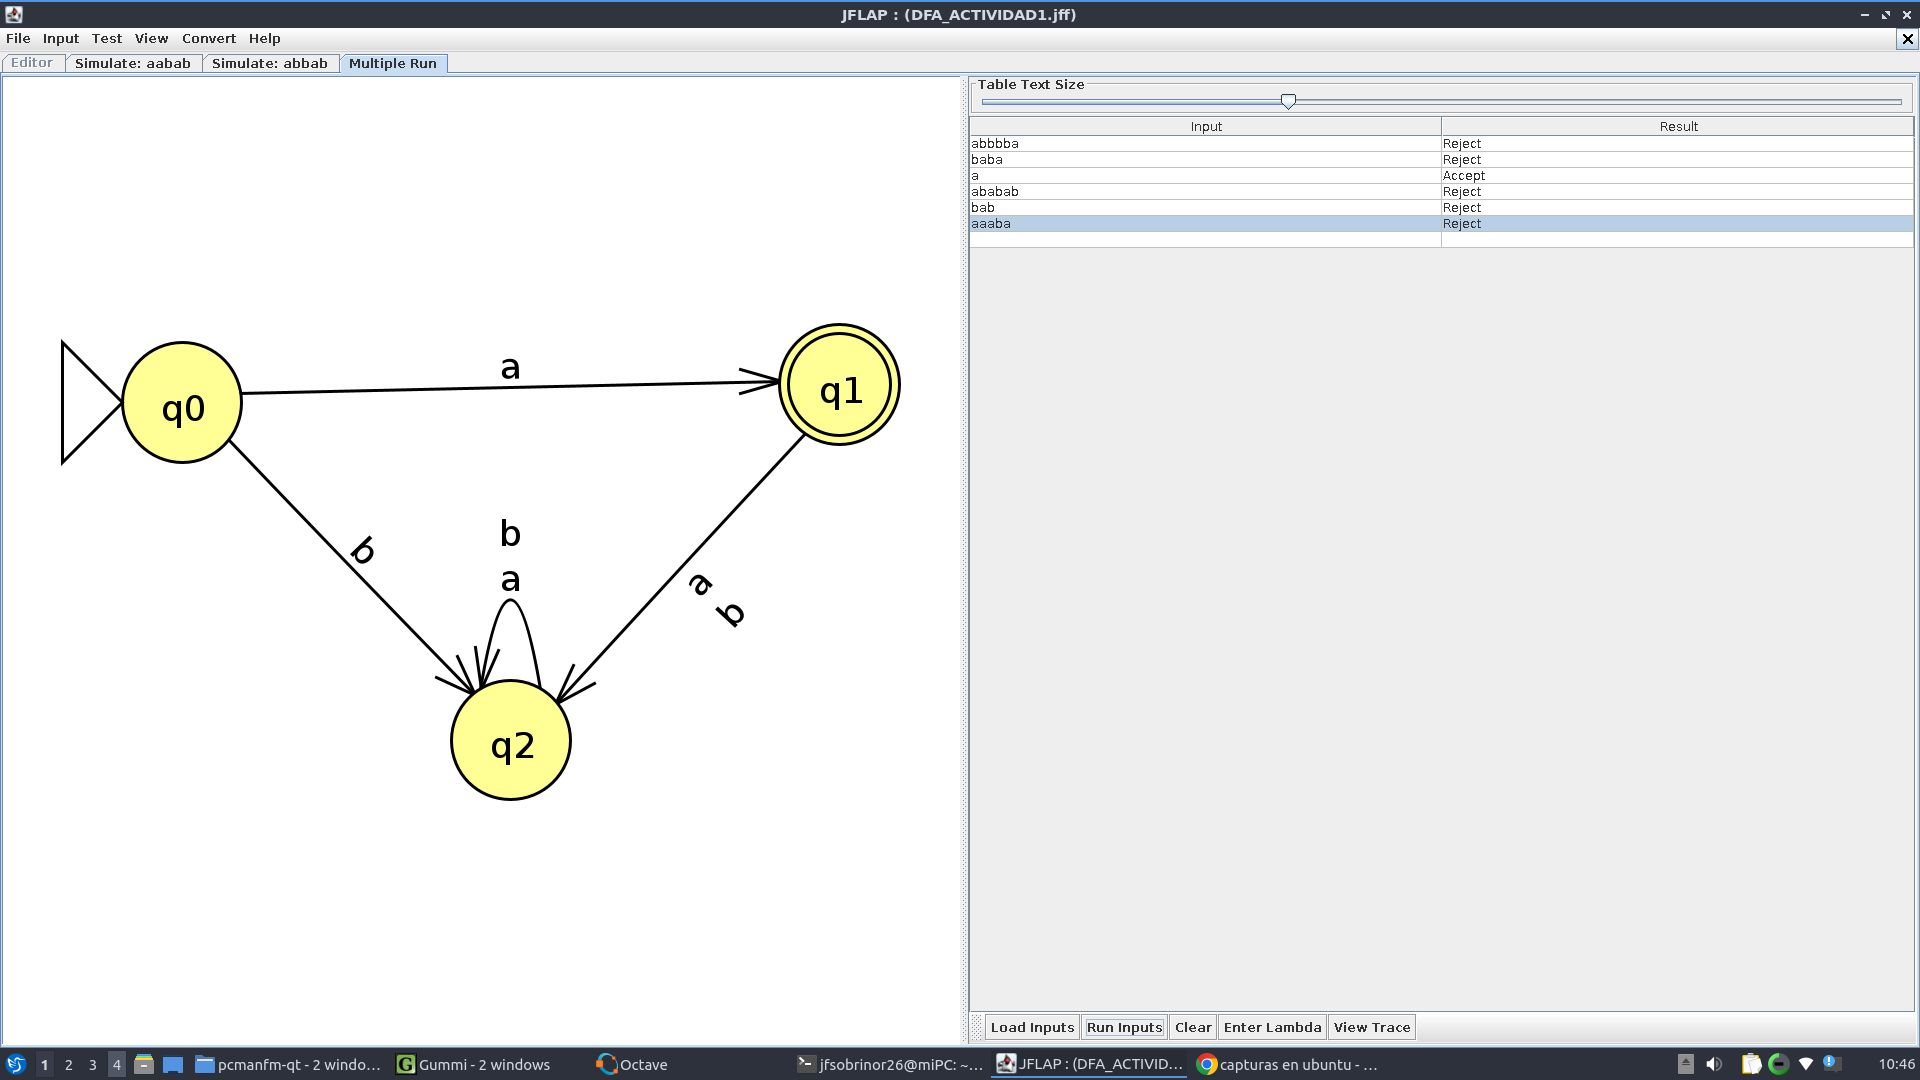
\includegraphics[scale=0.5]{DFA_ACTIVIDAD1}

\section*{2. Finite automaton in Octave:}
\subsection*{a. Open the Octave finiteautomata.m script and test it with the given
example (see script help) in the GitHub repository.\\
\\b. Specify in finiteautomata.json the automaton created in Activity 1
and test it with the script!\\}

Computation for a given finite automaton and string.
 The automaton can be either DFA or NFA, and it is defined
 in a JSON file, like this:\\
 \{\\
     "K" : ["q0", "q1", "q2"],\\
     "A" : ["a", "b"],\\
     "s" : "q0",\\
     "F" : ["q2"],\\
     "t" : [["q0", "a", "q1"],
            ["q1", "a", "q1"],
            ["q1", "b", "q2"],
            ["q2", "b", "q2"]]\\
   \}\\

   (a transition consuming the empty string: ["q1", "", "q2"])\\

For example:\\

octave:6 finiteautomata("aa*bb*", "ab", "LaTeX")
warning: strmatch is obsolete; use strncmp or strcmp instead\\

$M = ( {q_0, q_1, q_2}, {a, b}, q_0, {q_2}, {(q_0, a, q_1), (q_1, a, q_1), (q_1, b, q_2), (q_2, b, q_2)} )$

$w = ab$

$(q_0, ab) \vdash (q_1, b) \vdash (q_2, \varepsilon)$

$x \in L(M)$

\end{document}